\documentclass{standalone}

\usepackage{tikz}
\usepackage[T1]{fontenc}
\usepackage[tt=false, type1=true]{libertine}
\usepackage[varqu]{zi4}
\usepackage[libertine]{newtxmath}

\usetikzlibrary{shapes, positioning, calc}

\begin{document}

{\scriptsize
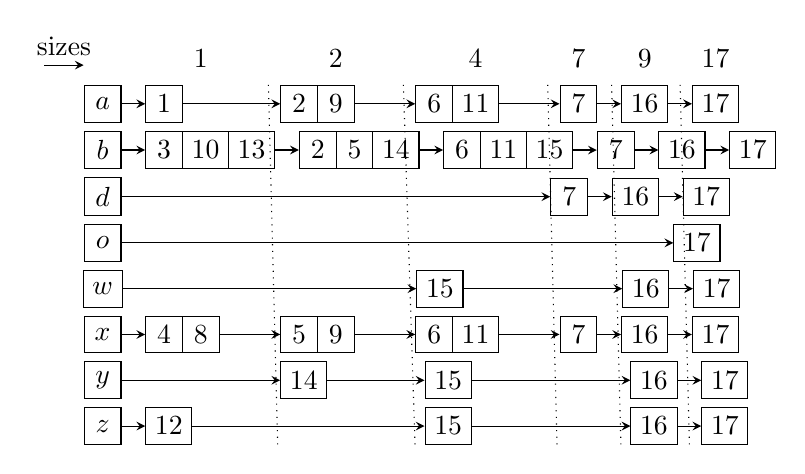
\begin{tikzpicture}
  \newcommand\listspacing{0.1}
  \newcommand\listpartspacing{0.3}
  \newcommand\arraypartspacing{0.015} % 0.03 for thick
  \newcommand\listdir{right}
  \newcommand\lbldir{below}
  \newcommand\listelemminwidth{0.4675cm }
  \newcommand\listelemminheight{0.4675cm}

  \tikzset{ptr/.style={->, >=stealth}}

  % inverted lists
  \node[draw, minimum width=\listelemminwidth, minimum height=\listelemminheight] at (0, 0) (il1) {$a$};
  \foreach \label/\ilid [count=\x from 1] in {b/2, d/3, o/4, w/5, x/6, y/7, z/8}{
    \node[draw, minimum width=\listelemminwidth, minimum height=\listelemminheight, \lbldir=\listspacing of il\x] (il\ilid) {$\label$};
  }

  % partition 1
  \node[draw, minimum width=\listelemminwidth, minimum height=\listelemminheight, \listdir=\listpartspacing of il1] (il1-1) {$1$};
  \foreach \poid/\idx [count=\x from 1] in {/2, /3}{
    \node[minimum width=\listelemminwidth, minimum height=\listelemminheight, \listdir=-\arraypartspacing of il1-\x] (il1-\idx) {$\poid$};
  }

  \node[draw, minimum width=\listelemminwidth, minimum height=\listelemminheight, \listdir=\listpartspacing of il2] (il2-1) {$3$};
  \foreach \poid/\idx [count=\x from 1] in {10/2, 13/3}{
    \node[draw, minimum width=\listelemminwidth, minimum height=\listelemminheight, \listdir=-\arraypartspacing of il2-\x] (il2-\idx) {$\poid$};
  }

  \node[minimum width=\listelemminwidth, minimum height=\listelemminheight, \listdir=\listpartspacing of il3] (il3-1) {};
  \foreach \poid/\idx [count=\x from 1] in {/2, /3}{
    \node[minimum width=\listelemminwidth, minimum height=\listelemminheight, \listdir=-\arraypartspacing of il3-\x] (il3-\idx) {$\poid$};
  }

  \node[minimum width=\listelemminwidth, minimum height=\listelemminheight, \listdir=\listpartspacing of il4] (il4-1) {};
  \foreach \poid/\idx [count=\x from 1] in {/2, /3}{
    \node[minimum width=\listelemminwidth, minimum height=\listelemminheight, \listdir=-\arraypartspacing of il4-\x] (il4-\idx) {$\poid$};
  }

  \node[minimum width=\listelemminwidth, minimum height=\listelemminheight, \listdir=\listpartspacing of il5] (il5-1) {};
  \foreach \poid/\idx [count=\x from 1] in {/2, /3}{
    \node[minimum width=\listelemminwidth, minimum height=\listelemminheight, \listdir=-\arraypartspacing of il5-\x] (il5-\idx) {$\poid$};
  }

  \node[draw, minimum width=\listelemminwidth, minimum height=\listelemminheight, \listdir=\listpartspacing of il6] (il6-1) {$4$};
  \foreach \poid/\idx [count=\x from 1] in {8/2}{
    \node[draw, minimum width=\listelemminwidth, minimum height=\listelemminheight, \listdir=-\arraypartspacing of il6-\x] (il6-\idx) {$\poid$};
  }
  \foreach \poid/\idx [count=\x from 2] in {/3}{
    \node[minimum width=\listelemminwidth, minimum height=\listelemminheight, \listdir=-\arraypartspacing of il6-\x] (il6-\idx) {$\poid$};
  }

  \node[minimum width=\listelemminwidth, minimum height=\listelemminheight, \listdir=\listpartspacing of il7] (il7-1) {};
  \foreach \poid/\idx [count=\x from 1] in {/2, /3}{
    \node[minimum width=\listelemminwidth, minimum height=\listelemminheight, \listdir=-\arraypartspacing of il7-\x] (il7-\idx) {$\poid$};
  }

  \node[draw, minimum width=\listelemminwidth, minimum height=\listelemminheight, \listdir=\listpartspacing of il8] (il8-1) {$12$};
  \foreach \poid/\idx [count=\x from 1] in {/2, /3}{
    \node[minimum width=\listelemminwidth, minimum height=\listelemminheight, \listdir=-\arraypartspacing of il8-\x] (il8-\idx) {$\poid$};
  }

  % partition 2
  \node[draw, minimum width=\listelemminwidth, minimum height=\listelemminheight, \listdir=\listpartspacing of il1-3] (il1-4) {$2$};
  \foreach \poid/\idx [count=\x from 4] in {9/5}{
    \node[draw, minimum width=\listelemminwidth, minimum height=\listelemminheight, \listdir=-\arraypartspacing of il1-\x] (il1-\idx) {$\poid$};
  }
  \foreach \poid/\idx [count=\x from 5] in {/6}{
    \node[minimum width=\listelemminwidth, minimum height=\listelemminheight, \listdir=-\arraypartspacing of il1-\x] (il1-\idx) {$\poid$};
  }

  \node[draw, minimum width=\listelemminwidth, minimum height=\listelemminheight, \listdir=\listpartspacing of il2-3] (il2-4) {$2$};
  \foreach \poid/\idx [count=\x from 4] in {5/5, 14/6}{
    \node[draw, minimum width=\listelemminwidth, minimum height=\listelemminheight, \listdir=-\arraypartspacing of il2-\x] (il2-\idx) {$\poid$};
  }

  \node[minimum width=\listelemminwidth, minimum height=\listelemminheight, \listdir=\listpartspacing of il3-3] (il3-4) {};
  \foreach \poid/\idx [count=\x from 4] in {/5, /6}{
    \node[minimum width=\listelemminwidth, minimum height=\listelemminheight, \listdir=-\arraypartspacing of il3-\x] (il3-\idx) {$\poid$};
  }

  \node[minimum width=\listelemminwidth, minimum height=\listelemminheight, \listdir=\listpartspacing of il4-3] (il4-4) {};
  \foreach \poid/\idx [count=\x from 4] in {/5, /6}{
    \node[minimum width=\listelemminwidth, minimum height=\listelemminheight, \listdir=-\arraypartspacing of il4-\x] (il4-\idx) {$\poid$};
  }

  \node[minimum width=\listelemminwidth, minimum height=\listelemminheight, \listdir=\listpartspacing of il5-3] (il5-4) {};
  \foreach \poid/\idx [count=\x from 4] in {/5, /6}{
    \node[minimum width=\listelemminwidth, minimum height=\listelemminheight, \listdir=-\arraypartspacing of il5-\x] (il5-\idx) {$\poid$};
  }

  \node[draw, minimum width=\listelemminwidth, minimum height=\listelemminheight, \listdir=\listpartspacing of il6-3] (il6-4) {$5$};
  \foreach \poid/\idx [count=\x from 4] in {9/5}{
    \node[draw, minimum width=\listelemminwidth, minimum height=\listelemminheight, \listdir=-\arraypartspacing of il6-\x] (il6-\idx) {$\poid$};
  }
  \foreach \poid/\idx [count=\x from 5] in {/6}{
    \node[minimum width=\listelemminwidth, minimum height=\listelemminheight, \listdir=-\arraypartspacing of il6-\x] (il6-\idx) {$\poid$};
  }

  \node[draw, minimum width=\listelemminwidth, minimum height=\listelemminheight, \listdir=\listpartspacing of il7-3] (il7-4) {$14$};
  \foreach \poid/\idx [count=\x from 4] in {/5, /6}{
    \node[minimum width=\listelemminwidth, minimum height=\listelemminheight, \listdir=-\arraypartspacing of il7-\x] (il7-\idx) {$\poid$};
  }

  \node[minimum width=\listelemminwidth, minimum height=\listelemminheight, \listdir=\listpartspacing of il8-3] (il8-4) {};
  \foreach \poid/\idx [count=\x from 4] in {/5, /6}{
    \node[minimum width=\listelemminwidth, minimum height=\listelemminheight, \listdir=-\arraypartspacing of il8-\x] (il8-\idx) {$\poid$};
  }

  % partition 3
  \node[draw, minimum width=\listelemminwidth, minimum height=\listelemminheight, \listdir=\listpartspacing of il1-6] (il1-7) {$6$};
  \foreach \poid/\idx [count=\x from 7] in {11/8}{
    \node[draw, minimum width=\listelemminwidth, minimum height=\listelemminheight, \listdir=-\arraypartspacing of il1-\x] (il1-\idx) {$\poid$};
  }
  \foreach \poid/\idx [count=\x from 8] in {/9}{
    \node[minimum width=\listelemminwidth, minimum height=\listelemminheight, \listdir=-\arraypartspacing of il1-\x] (il1-\idx) {$\poid$};
  }

  \node[draw, minimum width=\listelemminwidth, minimum height=\listelemminheight, \listdir=\listpartspacing of il2-6] (il2-7) {$6$};
  \foreach \poid/\idx [count=\x from 7] in {11/8, 15/9}{
    \node[draw, minimum width=\listelemminwidth, minimum height=\listelemminheight, \listdir=-\arraypartspacing of il2-\x] (il2-\idx) {$\poid$};
  }

  \node[minimum width=\listelemminwidth, minimum height=\listelemminheight, \listdir=\listpartspacing of il3-6] (il3-7) {};
  \foreach \poid/\idx [count=\x from 7] in {/8, /9}{
    \node[minimum width=\listelemminwidth, minimum height=\listelemminheight, \listdir=-\arraypartspacing of il3-\x] (il3-\idx) {$\poid$};
  }

  \node[minimum width=\listelemminwidth, minimum height=\listelemminheight, \listdir=\listpartspacing of il4-6] (il4-7) {};
  \foreach \poid/\idx [count=\x from 7] in {/8, /9}{
    \node[minimum width=\listelemminwidth, minimum height=\listelemminheight, \listdir=-\arraypartspacing of il4-\x] (il4-\idx) {$\poid$};
  }

  \node[draw, minimum width=\listelemminwidth, minimum height=\listelemminheight, \listdir=\listpartspacing of il5-6] (il5-7) {$15$};
  \foreach \poid/\idx [count=\x from 7] in {/8, /9}{
    \node[minimum width=\listelemminwidth, minimum height=\listelemminheight, \listdir=-\arraypartspacing of il5-\x] (il5-\idx) {$\poid$};
  }

  \node[draw, minimum width=\listelemminwidth, minimum height=\listelemminheight, \listdir=\listpartspacing of il6-6] (il6-7) {$6$};
  \foreach \poid/\idx [count=\x from 7] in {11/8}{
    \node[draw, minimum width=\listelemminwidth, minimum height=\listelemminheight, \listdir=-\arraypartspacing of il6-\x] (il6-\idx) {$\poid$};
  }
  \foreach \poid/\idx [count=\x from 8] in {/9}{
    \node[minimum width=\listelemminwidth, minimum height=\listelemminheight, \listdir=-\arraypartspacing of il6-\x] (il6-\idx) {$\poid$};
  }

  \node[draw, minimum width=\listelemminwidth, minimum height=\listelemminheight, \listdir=\listpartspacing of il7-6] (il7-7) {$15$};
  \foreach \poid/\idx [count=\x from 7] in {/8, /9}{
    \node[minimum width=\listelemminwidth, minimum height=\listelemminheight, \listdir=-\arraypartspacing of il7-\x] (il7-\idx) {$\poid$};
  }

  \node[draw, minimum width=\listelemminwidth, minimum height=\listelemminheight, \listdir=\listpartspacing of il8-6] (il8-7) {$15$};
  \foreach \poid/\idx [count=\x from 7] in {/8, /9}{
    \node[minimum width=\listelemminwidth, minimum height=\listelemminheight, \listdir=-\arraypartspacing of il8-\x] (il8-\idx) {$\poid$};
  }

  % partition 4
  \foreach \listid in {1, 2, 3, 6}{
    \node[draw, minimum width=\listelemminwidth, minimum height=\listelemminheight, \listdir=\listpartspacing of il\listid-9] (il\listid-10) {$7$};
  }

  \foreach \listid in {4, 5, 7, 8}{
    \node[minimum width=\listelemminwidth, minimum height=\listelemminheight, \listdir=\listpartspacing of il\listid-9] (il\listid-10) {};
  }

  % partition 5
  \foreach \listid in {1, 2, 3, 5, 6, 7, 8}{
    \node[draw, minimum width=\listelemminwidth, minimum height=\listelemminheight, \listdir=\listpartspacing of il\listid-10] (il\listid-11) {$16$};
  }

  \node[minimum width=\listelemminwidth, minimum height=\listelemminheight, \listdir=\listpartspacing of il4-10] (il4-11) {};

  % partition 6
  \foreach \listid in {1, ..., 8}{
    \node[draw, minimum width=\listelemminwidth, minimum height=\listelemminheight, \listdir=\listpartspacing of il\listid-11] (il\listid-12) {$17$};
  }

  % pointers
  \foreach \listid in {1, 2, 6, 8}{
    \draw[ptr] (il\listid) -- (il\listid-1);
  }
  \draw[ptr] (il3) -- (il3-10);
  \draw[ptr] (il4) -- (il4-12);
  \draw[ptr] (il5) -- (il5-7);
  \draw[ptr] (il7) -- (il7-4);

  \draw[ptr] (il1-1) -- (il1-4);
  \draw[ptr] (il2-3) -- (il2-4);
  \draw[ptr] (il6-2) -- (il6-4);
  \draw[ptr] (il8-1) -- (il8-7);

  \draw[ptr] (il1-5) -- (il1-7);
  \draw[ptr] (il2-6) -- (il2-7);
  \draw[ptr] (il6-5) -- (il6-7);
  \draw[ptr] (il7-4) -- (il7-7);

  \draw[ptr] (il1-8) -- (il1-10);
  \draw[ptr] (il2-9) -- (il2-10);
  \draw[ptr] (il5-7) -- (il5-11);
  \draw[ptr] (il6-8) -- (il6-10);
  \draw[ptr] (il7-7) -- (il7-11);
  \draw[ptr] (il8-7) -- (il8-11);

  \foreach \listid in {1, 2, 3, 6}{
    \draw[ptr] (il\listid-10) -- (il\listid-11);
  }

  \foreach \listid in {1, 2, 3, 5, 6, 7, 8}{
    \draw[ptr] (il\listid-11) -- (il\listid-12);
  }

  \draw[ptr] ($(il1.north west)+(-0.5,0.25)$) -- node[above] {sizes} ++(0.5, 0);

  % delimiters
  \foreach \a/\b in {3/4, 6/7, 9/10, 10/11, 11/12}{
    \draw[dotted] ($(il1-\a.north)!0.5!(il1-\b.north)$) -- ($(il8-\a.south)!0.5!(il8-\b.south)$);
  }

  % sizes
  \foreach \size/\elemid in {1/2, 2/5, 4/8, 7/10, 9/11, 17/12}{
    \node[above=\listspacing of il1-\elemid] {$\size$};
  }
\end{tikzpicture}}

\end{document}
